\chapter{Module development}
%============================================================================
\section{What is a module?}
\index{module mechanism}
OpenCms provides a module mechanism to add further functionality to the system. A module is a
dynamic extension of the system with XML templates and Java classes. A module can be uploaded,
installed and uninstalled from within the system. An example of a module is the backoffice part
of a discussion forum on a website that was created with OpenCms. You might wish to administer
the forums and comments from within OpenCms, i.e. delete or create database entries in a
specific, possibly external, database. You would include your pages with the dialogs and the
classes that implement this functionality in the module. A module can, but does not have to,
include Java classes, templates and documentation.

A module is a zip file that contains a number of other files (specified in detail below). This
module zip file can be uploaded using the OpenCms view {\name Administration}. You can upload the
file into OpenCms from your local machine or from the file system of the server where OpenCms runs.
The zip file will then be unpacked and it's content will be copied to the specified location
in the virtual file system. Information about these
files as well as other information about the module is stored in the system's registry,
which makes it possible to uninstall it. After the copy is finished, an event handler method
of one of the modules classes is invoked so that the module can do it's own initial work if desired.
Then the new module can be used as if it were a part of OpenCms.

\section{Creation of a module}

\begin{figure}[hbt]
\begin{center}
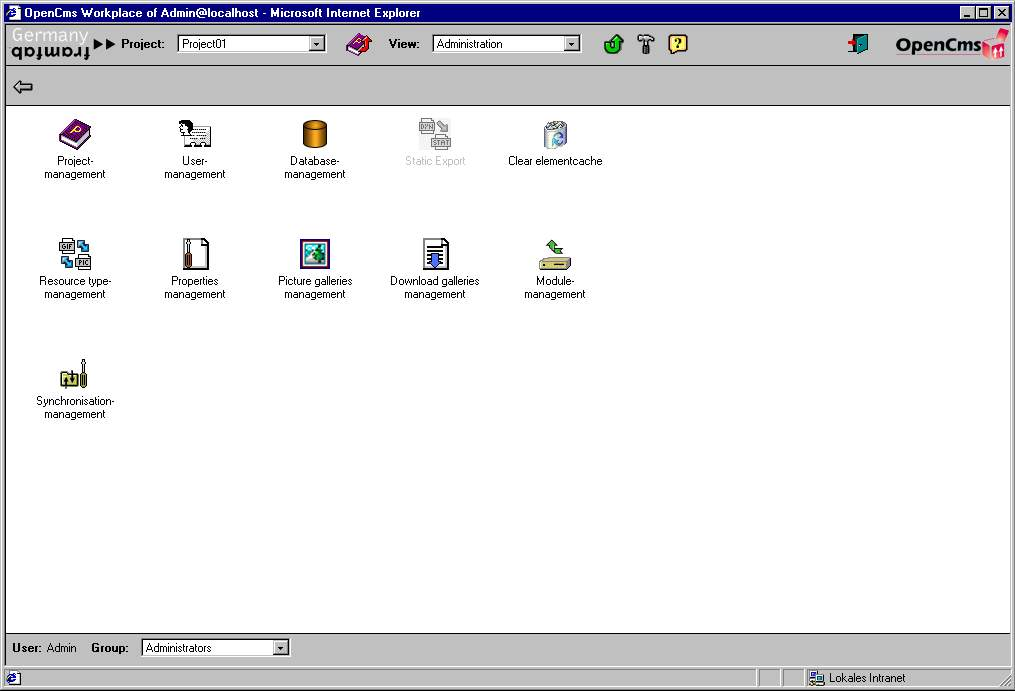
\includegraphics[width=\sgw]
                   {pics/templateMech/admin_point}
\caption[Administration view]
           {Administration view}
\label{AdView}
\end{center}
\end{figure}

The administration of modules is done under the administration view (see figure~\ref{AdView}).
Change to the administration view and then choose the item {\name Modulemanagement}.
In the next screen a list with the modules that are already installed is shown. Existing
modules can be deleted, administrated or exported. In this view existing modules can also
be added to the system (upload a module) or new modules can be created.

\begin{figure}[hbt]
\begin{center}
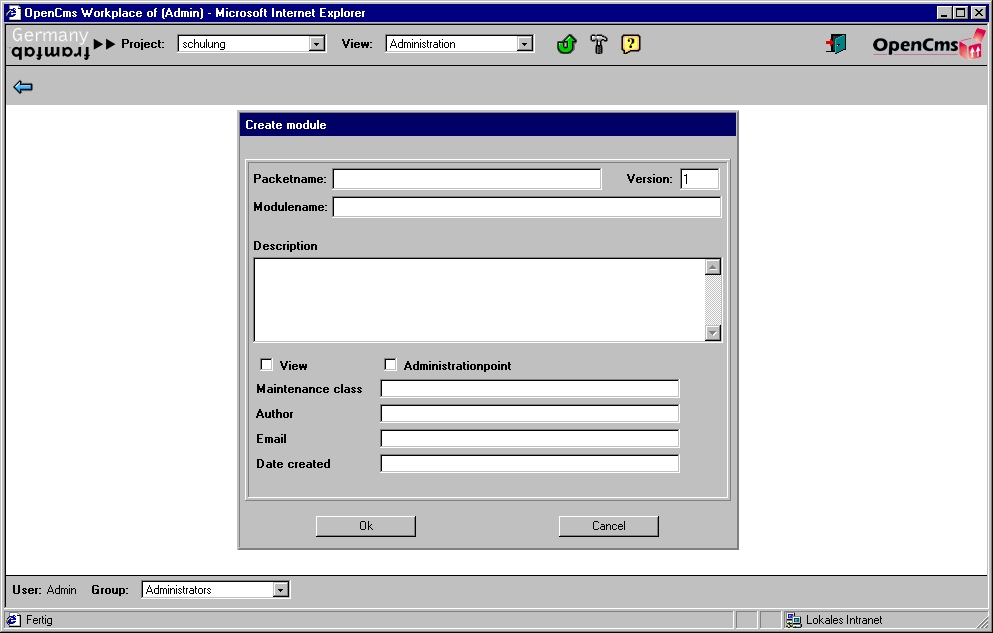
\includegraphics[width=\sgw]
                   {pics/templateMech/create_new}
\caption[Create a new module]
           {Create a new module}
\label{CreMod}
\end{center}
\end{figure}

The creation of a new module is done with the help of a wizard (figure~\ref{CreMod}).
Please notice that you have to be within an offline project that contains the root-folder
to be able to start the creation of a module.
All necessary information can be inserted in input fields and all but the packetname can
be changed later, if necessary. The following properties of a module can be defined:

\begin{itemize}
\item[-]The {\bf Packetname} determines a unique name of the module.
It has to be a name that follows the Java naming conventions for package names.
For example, your module could be called {\name com.opencms.mymodule}. This name has to be
determined at first and can�t be changed after the module was  created. Normally your module
contains templates and Java classes as well. Please keep in mind that the name of your module and the
name of your Java package in your development environment have to be exactly the same. Thus,
your classes for the above example should reside in the package {\name com.opencms.mymodule}.

\item[-]The {\bf Modulename} can be freely chosen and should be a descriptive name for the module. 

\item[-]The item {\bf Version} is the version number of the module as an integer. 

\item[-]The checkbox {\bf View} has to be chosen if the module should add a new view 
to OpenCms (a new entry in the view select box).

\item[-]The module can also provide a new administrationpoint. 
In this case the checkbox {\bf Administrationpoint} has to be chosen. 

\item[-]In the field {\bf Maintenance class} you can specify a class (with its fully-qualified class name) 
that handles events like deleting a module, uploading a module and changing of the module parameters. This
class has to implement certain methods to handle these events. There are three methods you may use: 

public static void moduleWasUploaded(CmsObject cms)

public static void moduleParameterWasUpdated(CmsObject cms)

public static void moduleWasDeleted(CmsObject cms).

OpenCms trys to call these methodes when
the module is imported, a module parameter is changed or the module is deleted from the system. 

\item[-] The fields {\bf Author} and {\bf Email} can be used to provide information about the author
of the module.

\item[-] The field {\bf Date created} will be filled with the current date when creating the module but
can also be changed later.
\end{itemize}

\begin{figure}[hbt]
\begin{center}
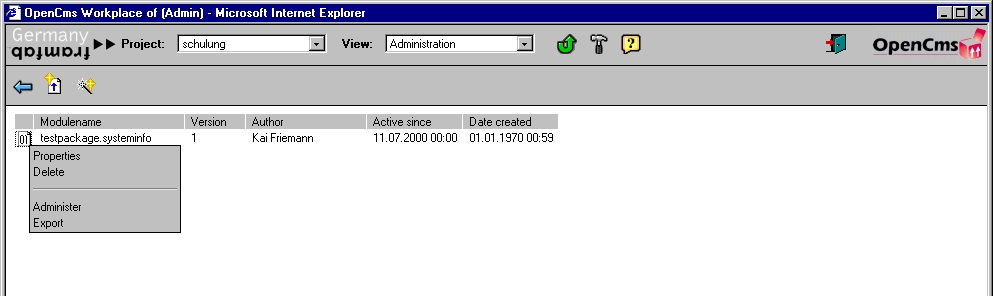
\includegraphics[width=\sgw]
                   {pics/templateMech/mod_list}
\caption[The list of modules]
           {The list of modules}
\label{ModList}
\end{center}
\end{figure}

Some more details can be determined after creating the module. You can specify 
dependencies when choosing the item {\name administer} from the context menue of your
module.
It is possible that your module depends on several other  modules, that might have certain
version numbers. In this case these dependencies can be specified after the module has been
created (figure~\ref{deps}). If you define these dependencies OpenCms checks whether all
dependencies are fullfilled when you upload or delete a module.

\begin{figure}[hbt]
\begin{center}
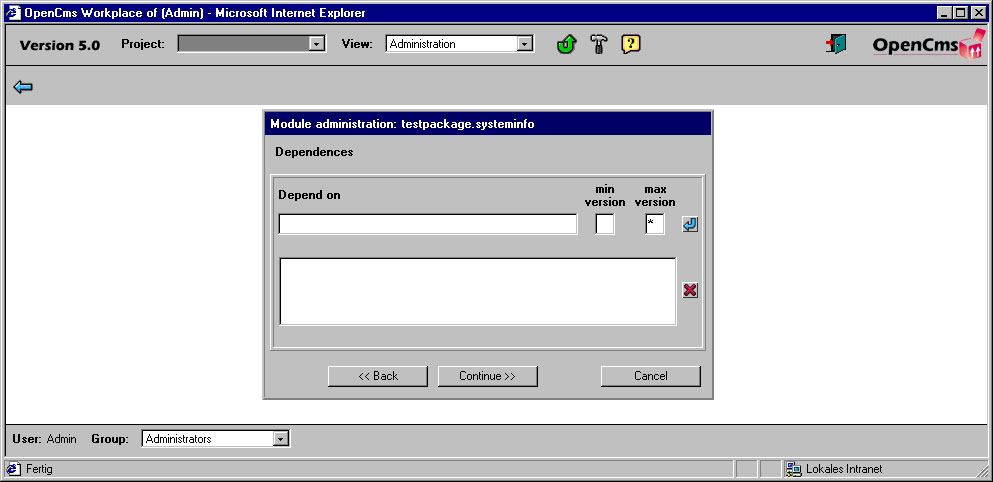
\includegraphics[width=\sgw]
                   {pics/templateMech/admin_2}
\caption[Dependencies to other modules]
           {Dependencies to other modules}
\label{deps}
\end{center}
\end{figure}

The module mechanism uses the module's name (the package name) to create certain directories. One important thing
when handling modules is to follow the recommended way of creating and storing files and folders.
The module mechanism creates some new folder-trees.
A directory {\dir package\_name/} is created in the directory {\dir /moduledemos/} for every new module.
In this directory should be a demoversion of your module. Normally this would be a demo page
that makes usage of the functionality you implemented. The entry point of your demo should always be
a file called {\name index.html}.
Another directory {\dir package\_name/} is created within the {\dir /system/modules/} directroy.
This directory
contains certain sub-directories that have been created by the module mechanism. A subdirectory
{\name administration} is created if you have chosen your module to provide a new administration
item in the administration view.

\subsubsection{Mastertemplates}

All master templates that belong to your module have to be stored in the\\
{\dir /system/modules/package\_name/templates/} directory. You can choose these mastertemplates
from a select box when you are creating a new page. 
Other (sub-)templates that are used by your module should be stored inside another directory
within your module subtree. Only files that lie within your module subtrees can be found by
OpenCms when you export your module.

\subsubsection{Classes that correspond to the pages}

Your Java classes, i.e the byte code, are also resources in the OpenCms system.
The module mechanism creates a further directory for these classes. For this reason, the name
of your module (e.g. com.opencms.examples.newsmodule) is splitted into subdirectories
(e.g. {\dir /com/opencms/examples/newsmodule/} ). You can use a JAR file, a zip file or class files.
While developing your module, you can leave the classes in your local file system within your
classpath. It is only important to upload the classes when you finish (and export) your module.
A mechanism to "synchronize" (or upload) the classes in an easy way will be discussed in chapter
~\ref{synchronization} (page \pageref{synchronization}).

\subsubsection{Adding a new administration item}

When you change to the administration view, a number of icons such as
{\name Project Administration} and
{\name User Administration} are displayed. This section describes how to add your own item. You
will need an icon in the form of a GIF file that fits in terms of size and style. If you would
like to have a variant for an inactive item, the file should have the same name with the
addition of {\name \_in} for inactive at the end of the file name, before the extension
{\name .gif.} Put
this image in the folder {\dir /system /modules/package\_name/pics/} and ensure that it's owner
and group are one of the three standard users and groups.
For every item that should be displayed, a new directory (for example {\name mymodule}) has to be
created in the {\dir /system /modules/package\_name/administration/} directory.
Then give the folder

{\dir /system /modules/package\_name/administration/mymodule/}

new properties by selecting 'Properties' from the context menue:

\begin{table}\begin{center}
\begin{tabular}{|l|p{0.75\linewidth}|}
\hline
{\bf property} & {\bf description} \\ \hline 
NavPos  &
This real number determines the order of the icons in the administration view. The
icons are ordered by increasing NavPos. To add your icon at the end select a value greater than the highest of all
NavPos values in the other folders in the directory {\dir /system/workplace/administration/}.\\ \hline
NavText &
The tag for the subtitle of the icon in the language files you provide. You will
have to provide one or more language files with this subtitle in each language. The tag should
be the same in all language files.\\ \hline
Title  &
The name of the GIF file of the icon that is used in the Administration view
without the extension {\name .gif}.\\ \hline
\index{visiblemethod}  visiblemethod &
Visiblemethod is a method that returns a boolean value. It returns true when the
icon is displayed to the current user in the current project. If it returns false, the icon is
not displayed. If you do not specify this method the icon will always be visible. You can enter
the name of the method here. When creating the new property you have to determine a method
(including the fully-qulified classname) under the item {\name Enter Property value}. See folders in the
{\dir /system/workplace/administration/} directory for an example.\\ \hline
\index{activemethod} activemethod &
Activemethod is a method that returns a boolean value. It returns true when
the icon is active, i.e. clickable. If false, the icon is still displayed but in an inactive
style, and without a link to the icon. If you do not specify this method the icon will always
be active. You can enter the name of the method here. When creating the new property you have
to determine a method (including the fully-qualified classname) under the item {\name Enter Property value}. 
See folders in the {\dir /system/workplace/administration/} directory for an example.\\
\hline
\end{tabular}
\caption[Properties] {Properties}
\label{direct}\end{center}
\end{table}


Here is an example for the properties:\\
\begin{xml}
NavPos = 7\\
NavText = mymodule.administration.icon.paybyclick\\
Title = paybyclick\\
visiblemethod = com.opencms.workplace.CmsWorkplaceDefault.isNotOnlineProject\\
\end{xml}

In the folder {\name mymodule}, create a page with the name index.html. This is the page that will be
displayed when the new item is clicked.

You also have the ability to display several administration items when your item is clicked,
as is currently done for the
{\name User Administration} and {\name Project Administration} items. Simply
add new subfolders in the
{\dir /system/modules/package\_name/ad\-minis\-tration/my\-module/} directory, give
them the same properties as above, and add icons and an index.html page to each subfolder. Please
notice that every directory that is created within the {\dir /administration/} directory will be
added as an administration item frome the module mechanism and an error will occur if you add
directories here that don�t follow these conventions.
In the administration view there is an additional frame {\name admin\_head} for navigation just below
the toolbar. If you only want to use the standard frame with the blue back button then let this
frame be updated when your {\name index.html} is displayed by adding the following onLoad javascipt to
your body tag: 

{\code
<body onLoad="window.top.body.admin\_head.location.href='[path to the /sys\-tem/\\
workplace/action folder]/administration\_head.html';"> }

Or create your own {\name admin\_head} frame. You might want to look at the picture or download
galleries that you can use as examples.

\subsubsection{Adding a new view}

It is also possible to add an entry in the view select box, similar to the entries for
{\name Explorer}, or {\name Administration}. If you have activated the checkbox
{\name view} when you created the
module, a directory with the name {\name view} has automatically been created within the
{\dir /system/modules/package\_name/} directory. In this case you have to put a file with the
name {\name index.html} into this directory. This is the HTML page that should be displayed when your
view has been selected from the select box. Of course there has to be a corresponding tag in
the language file.

\subsubsection{Language Files}
\index{Language Files}
OpenCms supports multiple languages on the workplace, and it is possible to run several
languages on the same server simultaneously. Users can select their preferred language by
clicking on the hammer icon and selecting the start settings. Currently we only support German
and English, but it is easy to write language files in another language by copying existing
files and translating them tag by tag. The developers welcome any suggestions and contributions
you may wish to make about language files. Please send your ideas to contributions@opencms.org.
To make multiple languages possible at all it is important that you put every piece of text that
appears on the workplace in the language file(s) of your module. This might seem long winded but
not doing this means that translating your module to another language will be very time and cost
intensive. Make sure to include the English version of your language file. The language files
are XML files that are stored in the folder {\dir /system/modules/package\_name/language/}.
This folder
contains subfolders for each supported language (de, uk). The language names correspond to their
top-level domain names. In each of these subfolders there is a language file
(e.g. {\name mymodule\_uk})
for the module. The name should be the same as the packagename of the module, say
{\code com.opencms.mymodule}, followed by an underscore and the language code.

Example:

Create an English language file
\begin{xml}
/system/modules/com.opencms.mymodule/language/uk/com.opencms.mymodule\_uk
\end{xml}

that looks like this:
\begin{xml}
<?xml version="1.0" encoding="ISO-8859-1"?>\\
<LANGUAGE>\\
\xtaba   <name>English</name>\\
\xtaba   <com\_opencms\_mymodule>\\
\xtabb     <!-- fill in your tags here -->\\
\xtaba   </com\_opencms\_mymodule>\\
</LANGUAGE>\\
\end{xml}

Make sure to include your modulename at the top level because all of the language files that
belong to the same language are merged, and doing this avoids name clashing. Within the
language file, dots (".") inside the modulename have to be replaced with underscores ("\_").

\subsubsection{Documentation}
\index{Documentation}
Modules should be well documented. The module mechanism creates two folders.
The directory {\dir /system/modules/package\_name/doc/} is created to hold some textual
documentation. A file {\name index.html} should be placed here.
The directory {\dir /moduledemos/package\_name/} is automatically as well. Inside this
directroy has to be a demo of the module.
The demo is a template, that uses all features of the module in
a simple way.
If you create a new page within this demo directory, the corresponding content file is created
inside the {\dir /system/bodies/} directory.
These files are part of the module and exported together with the other resources of the module.

\subsubsection{Directories}

Here is a short overview of the directories that are created by the module mechanism:

\begin{xml}
/moduledemos/com.opencms.mymodule\\
/system/modules/com.opencms.mymodule/\\
\xtaba                    /administration \\
\xtabb                         /view \\
\xtabb                         /templates \\
\xtabb                         /frametemplates \\
\xtabb                         /contenttemplates \\
\xtabb                         /default\_bodies \\
\xtabb                         /elements \\
\xtabb                         /language \\
\xtabc                              /de \\
\xtabc                              /uk \\
\xtabb                         /doc\\
/system/classes/com/opencms/mymodule\\
\end{xml}